\chapter{SOLUCI\'ON DEFINITIVA}

\section{CONEXI\'ON PARA CADA UNA DE LAS SEDES}
\section{MARCO CONCEPTUAL}
\subsubsection{ Modelo de dise\~no jer\'arquico}
Se separa en 3 capas:
\begin{definicion}[]
{
\begin{enumerate}[label=\itembolasazules{}]
\item \textbf{Capa de acceso:} Es la interfaz con los dispositivos finales. Esta capa de acceso puede incluir routers, switches, puentes, hubs y puntos de acceso inal\'ambricos. Los switches de la capa de acceso facilitan la conexi\'on de los dispositivos de nodo final a la red. Por esta raz\'on, necesitan admitir caracter\'isticas como seguridad de puerto (el switch decide cu\'antos y qu\'e dispositivos se permiten conectar), VLAN, Fast Ethernet/Gigabit Ethernet, PoE, QOS y agregado de enlaces.
\\
En el caso planteado se har\'a uso de switchs de capa 2 para cumplir esta tarea.
\item\textbf{ Capa de distribuci\'on: } Controla el flujo de tr\'afico de la red con el uso de pol\'iticas y traza los dominios de broadcast al realizar el enrutamiento de las funciones entre las VLANs definidas en la capa de acceso. Presentan disponibilidad y redundancia altas para asegurar la fiabilidad. Los switches de capa de distribuci\'on recopilan los datos de todos los switches de capa de acceso y los env\'ian a los switches de capa n\'ucleo. 
\\
En el caso de estudio presentado se har\'a uso de switch de capa 3.
\item \textbf{Capa n\'ucleo:} Interconecta los dispositivos de la capa de distribuci\'on y puede conectarse a los recursos de Internet. El n\'ucleo debe estar disponible y ser redundante. Suelen contar con opciones de refrigeraci\'on más sofisticadas (alcanzan mayor temperatura por la carga de trabajo), con hardware que permite el cambio en caliente y QOS.
\\
Para el caso presentado se har\'a uso de routers de capa 3
\end{enumerate}
}
\end{definicion}}

\begin{center}
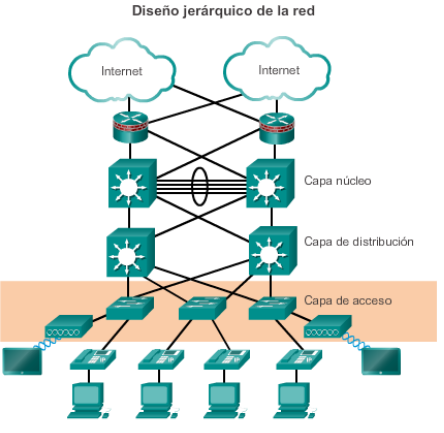
\includegraphics[scale=0.60]{jerarquico}
\end{center}

\subsubsection{ Modelo de n\'ucleo colapsado}
\begin{definicion}[]
{
 combina la capa de distribuci\'on y la capa n\'ucleo
 }
\end{definicion}
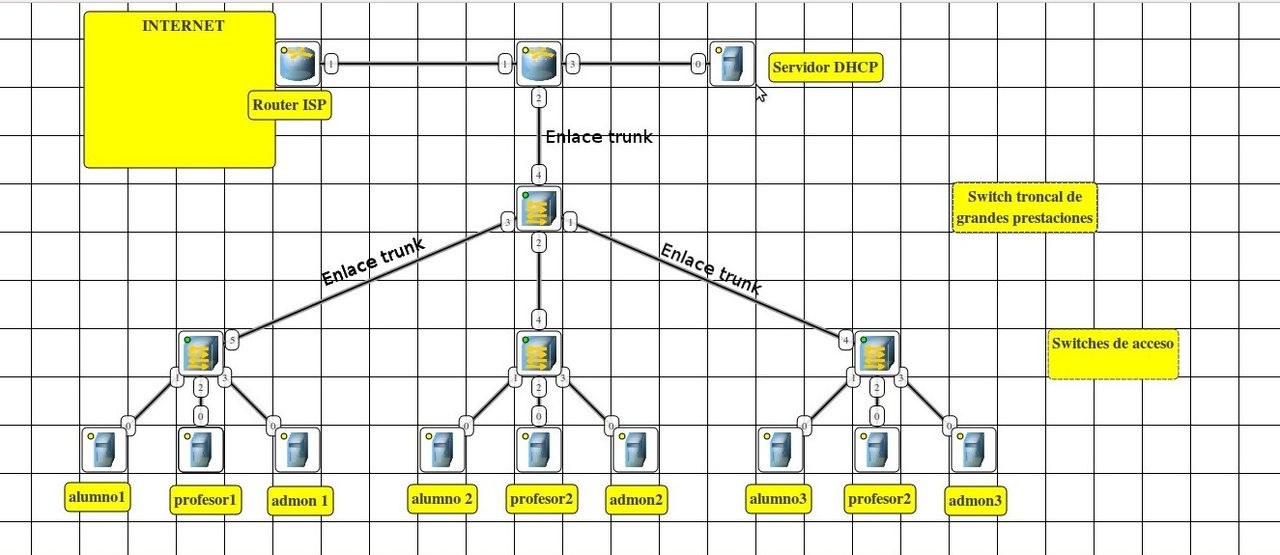
\includegraphics[scale=0.33]{colapsada}

El modelo de dise\~no jer\'arquico es el que implementaremos en el proyecto presente.

\section{Tipo de direcci\'on IP p\'ublica}

\begin{definicion}[]
{
 Para la salida del router usaremos esta ip publica la cual permitir\'a brindar seguridad a nuestra red; para ello realizaremos una configuraci\'on NAT en los routers externos.
 \\
 Usaremos una ip p\'ublica de clase B para este ejemplo: 192.100.3.0\\
A partir de ella realizando la segmentaci\'on obtendremos las ips de cada lan.
 }
\end{definicion}

\section{estructura de conexi\'on para la interconexi\'on entre routers}
Se har\'a uso de una conexi\'on serial.\\
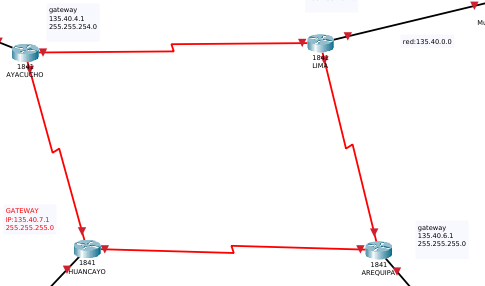
\includegraphics[scale=0.5]{img/router.png} 

\section{segmentaci\'on de subredes IP}

\subsection{Sede Central Ayacucho}
Usaremos la ip privada: 192.100.3.0
\\
Para hallar usaremos el m\'etodo de VLSM, con el tercer y cuarto octeto. \\

\\
Entonces tenemos:

IP: 192.100.3.0
\\
\textbf{SUMAMOS LOS COMPUTADORES QUE SE REQUIERE DE CADA SUCURSAL:}
\\

\begin{definicion}[]
{
\begin{enumerate}[label=\itembolasazules{}]
\item Sede Lima: 1000 computadoras
\item Sede Ayacucho: 400 computadoras
\item Sede Arequipa: 220 computadoras
\item Sede Huanta: 180 computadoras\\
\end{enumerate}
}
\end{definicion}}

Para poder hacer la segmentaci\'on necesitamos: \\
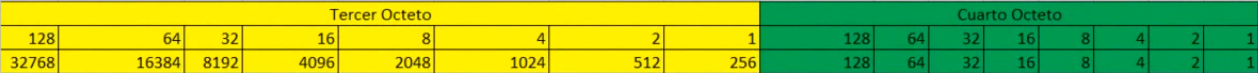
\includegraphics[scale=0.35]{img/octetos.png}
sabemos que la primera subred es la que nos dan por defecto entonces: \\

\begin{table}[htbp]
\begin{tabular}{@{}llllllll@{}}
\toprule
\rowcolor[HTML]{32CB00} 
\textbf{subred} & \textbf{host} & \textbf{n} & \textbf{direccion de sub red} & \textbf{rango ip} & \textbf{gateway} & \textbf{mascara} & \textbf{/MSR} \\ \midrule
lima            & 1000          &            & 135.40.0.0                    &                   &                  &                  &               \\ \bottomrule
\end{tabular}
\end{table}

Para hallar la siguiente sub red: vemos que requiere 1000 host buscamos este numero en la tabla o un valor mayor.
\\
En este caso para 1000 es 1024; por lo tanto n= 4\\
Quiere decir que la siguiente sub red tendr\'a un salto de 4, asi tenemos:

\begin{table}[htbp]
\begin{tabular}{@{}llllllll@{}}
\toprule
\rowcolor[HTML]{32CB00} 
\textbf{subred} & \textbf{host} & \textbf{n} & \textbf{direccion de sub red} & \textbf{rango ip} & \textbf{gateway} & \textbf{mascara} & \textbf{/MSR} \\ \midrule
lima            & 1000          & 4          & 135.40.0.0                    &                   &                  &                  &               \\ \midrule
Ayacucho        & 400           &            & 135.40.4.0                    &                   &                  &                  &              
\end{tabular}
\end{table}

realizamos el mismo paso para los dem\'as:\\
y nos quedaria:
\begin{table}[htbp]
\begin{tabular}{@{}llllllll@{}}
\toprule
\rowcolor[HTML]{32CB00} 
\multicolumn{1}{|l|}{\cellcolor[HTML]{32CB00}\textbf{subred}} & \multicolumn{1}{l|}{\cellcolor[HTML]{32CB00}\textbf{host}} & \multicolumn{1}{l|}{\cellcolor[HTML]{32CB00}\textbf{n}} & \multicolumn{1}{l|}{\cellcolor[HTML]{32CB00}\textbf{direccion de sub red}} & \multicolumn{1}{l|}{\cellcolor[HTML]{32CB00}\textbf{rango ip}} & \multicolumn{1}{l|}{\cellcolor[HTML]{32CB00}\textbf{gateway}} & \multicolumn{1}{l|}{\cellcolor[HTML]{32CB00}\textbf{mascara}} & \multicolumn{1}{l|}{\cellcolor[HTML]{32CB00}\textbf{/MSR}} \\ \midrule
\multicolumn{1}{|l|}{lima}                                    & \multicolumn{1}{l|}{1000}                                  & \multicolumn{1}{l|}{4}                                  & \multicolumn{1}{l|}{135.40.0.0}                                            & \multicolumn{1}{l|}{}                                          & \multicolumn{1}{l|}{}                                         & \multicolumn{1}{l|}{}                                         & \multicolumn{1}{l|}{}                                      \\ \midrule
\multicolumn{1}{|l|}{Ayacucho}                                & \multicolumn{1}{l|}{400}                                   & \multicolumn{1}{l|}{2}                                  & \multicolumn{1}{l|}{135.40.4.0}                                            & \multicolumn{1}{l|}{}                                          & \multicolumn{1}{l|}{}                                         & \multicolumn{1}{l|}{}                                         & \multicolumn{1}{l|}{}                                      \\ \midrule
\multicolumn{1}{|l|}{Arequipa}                                & \multicolumn{1}{l|}{220}                                   & \multicolumn{1}{l|}{1}                                  & \multicolumn{1}{l|}{135.40.6.0}                                            & \multicolumn{1}{l|}{}                                          & \multicolumn{1}{l|}{}                                         & \multicolumn{1}{l|}{}                                         & \multicolumn{1}{l|}{}                                      \\ \midrule
\multicolumn{1}{|l|}{Huancayo}                                & \multicolumn{1}{l|}{180}                                   & \multicolumn{1}{l|}{1}                                  & \multicolumn{1}{l|}{135.40.7.0}                                            & \multicolumn{1}{l|}{}                                          & \multicolumn{1}{l|}{}                                         & \multicolumn{1}{l|}{}                                         & \multicolumn{1}{l|}{}                                      \\ \midrule
                                                              &                                                            &                                                         & 135.40.8.0                                                                 &                                                                &                                                               &                                                               &                                                           
\end{tabular}
\end{table}

Para hallar la mascara de sub red lo que hacemos es sumar todos los n\'umeros que esten a la derecha de n incluido n; es decir para la sub red 135.40.0.0 n=4
entonces sumamos: \\
128+64+32+16+8+4 = 252\\
Entonces la MSR seria = 255.255.252.0\\
sacamos el /msr como hasta 4 ocupa 6 bits + los 16 bits del primer y segundo octeto ser\'ia = 22; asi tenemos:

\begin{table}[htbp]
\begin{tabular}{@{}llllllll@{}}
\toprule
\rowcolor[HTML]{32CB00} 
\multicolumn{1}{|l|}{\cellcolor[HTML]{32CB00}\textbf{subred}} & \multicolumn{1}{l|}{\cellcolor[HTML]{32CB00}\textbf{host}} & \multicolumn{1}{l|}{\cellcolor[HTML]{32CB00}\textbf{n}} & \multicolumn{1}{l|}{\cellcolor[HTML]{32CB00}\textbf{direccion de sub red}} & \multicolumn{1}{l|}{\cellcolor[HTML]{32CB00}\textbf{rango ip}} & \multicolumn{1}{l|}{\cellcolor[HTML]{32CB00}\textbf{gateway}} & \multicolumn{1}{l|}{\cellcolor[HTML]{32CB00}\textbf{mascara}} & \multicolumn{1}{l|}{\cellcolor[HTML]{32CB00}\textbf{/MSR}} \\ \midrule
\multicolumn{1}{|l|}{lima}                                    & \multicolumn{1}{l|}{1000}                                  & \multicolumn{1}{l|}{4}                                  & \multicolumn{1}{l|}{135.40.0.0}                                            & \multicolumn{1}{l|}{}                                          & \multicolumn{1}{l|}{}                                         & \multicolumn{1}{l|}{255.255.252.0}                            & \multicolumn{1}{l|}{/22}                                   \\ \midrule
\multicolumn{1}{|l|}{Ayacucho}                                & \multicolumn{1}{l|}{400}                                   & \multicolumn{1}{l|}{2}                                  & \multicolumn{1}{l|}{135.40.4.0}                                            & \multicolumn{1}{l|}{}                                          & \multicolumn{1}{l|}{}                                         & \multicolumn{1}{l|}{}                                         & \multicolumn{1}{l|}{}                                      \\ \midrule
\multicolumn{1}{|l|}{Arequipa}                                & \multicolumn{1}{l|}{220}                                   & \multicolumn{1}{l|}{1}                                  & \multicolumn{1}{l|}{135.40.6.0}                                            & \multicolumn{1}{l|}{}                                          & \multicolumn{1}{l|}{}                                         & \multicolumn{1}{l|}{}                                         & \multicolumn{1}{l|}{}                                      \\ \midrule
\multicolumn{1}{|l|}{Huancayo}                                & \multicolumn{1}{l|}{180}                                   & \multicolumn{1}{l|}{1}                                  & \multicolumn{1}{l|}{135.40.7.0}                                            & \multicolumn{1}{l|}{}                                          & \multicolumn{1}{l|}{}                                         & \multicolumn{1}{l|}{}                                         & \multicolumn{1}{l|}{}                                      \\ \midrule
                                                              &                                                            &                                                         & 135.40.8.0                                                                 &                                                                &                                                               &                                                               &                                                           
\end{tabular}
\end{table}

repetimos para todas las sub redes:

\begin{table}[htbp]
\begin{tabular}{@{}llllllll@{}}
\toprule
\rowcolor[HTML]{32CB00} 
\multicolumn{1}{|l|}{\cellcolor[HTML]{32CB00}\textbf{subred}} & \multicolumn{1}{l|}{\cellcolor[HTML]{32CB00}\textbf{host}} & \multicolumn{1}{l|}{\cellcolor[HTML]{32CB00}\textbf{n}} & \multicolumn{1}{l|}{\cellcolor[HTML]{32CB00}\textbf{direccion de sub red}} & \multicolumn{1}{l|}{\cellcolor[HTML]{32CB00}\textbf{rango ip}} & \multicolumn{1}{l|}{\cellcolor[HTML]{32CB00}\textbf{gateway}} & \multicolumn{1}{l|}{\cellcolor[HTML]{32CB00}\textbf{mascara}} & \multicolumn{1}{l|}{\cellcolor[HTML]{32CB00}\textbf{/MSR}} \\ \midrule
\multicolumn{1}{|l|}{lima}                                    & \multicolumn{1}{l|}{1000}                                  & \multicolumn{1}{l|}{4}                                  & \multicolumn{1}{l|}{135.40.0.0}                                            & \multicolumn{1}{l|}{}                                          & \multicolumn{1}{l|}{}                                         & \multicolumn{1}{l|}{255.255.252.0}                            & \multicolumn{1}{l|}{/22}                                   \\ \midrule
\multicolumn{1}{|l|}{Ayacucho}                                & \multicolumn{1}{l|}{400}                                   & \multicolumn{1}{l|}{2}                                  & \multicolumn{1}{l|}{135.40.4.0}                                            & \multicolumn{1}{l|}{}                                          & \multicolumn{1}{l|}{}                                         & \multicolumn{1}{l|}{255.255.254.0}                            & \multicolumn{1}{l|}{/23}                                   \\ \midrule
\multicolumn{1}{|l|}{Arequipa}                                & \multicolumn{1}{l|}{220}                                   & \multicolumn{1}{l|}{1}                                  & \multicolumn{1}{l|}{135.40.6.0}                                            & \multicolumn{1}{l|}{}                                          & \multicolumn{1}{l|}{}                                         & \multicolumn{1}{l|}{255.255.255.0}                            & \multicolumn{1}{l|}{/24}                                   \\ \midrule
\multicolumn{1}{|l|}{Huancayo}                                & \multicolumn{1}{l|}{180}                                   & \multicolumn{1}{l|}{1}                                  & \multicolumn{1}{l|}{135.40.7.0}                                            & \multicolumn{1}{l|}{}                                          & \multicolumn{1}{l|}{}                                         & \multicolumn{1}{l|}{255.255.255.0}                            & \multicolumn{1}{l|}{/24}                                   \\ \midrule
                                                              &                                                            &                                                         & 135.40.8.0                                                                 &                                                                &                                                               &                                                               &                                                           
\end{tabular}
\end{table}

Para hallar el rango de IP para 135.40.0.0 seria 135.40.0.1 y para calcular la ultima ip tenemos que la siguiete sub red es 135.4.4.0 entonces el ultimo ip tiene que ser 135.4.3.254; el 3 sale de restar menos 1 al 2 bit de 135.4.4.0 y 254 sale ya que podemos tener 255 pero es reservado para el broadcast por ello solo es hasta 254.
\\
Sabemos que el gateway va ser la primera ip es decir 135.40.0.1 y el broadcast el ultimo +1 es decir 135.40.3.255; y asi va ser para todos;



\begin{table}[htbp]
\begin{tabular}{@{}lllllll@{}}
\toprule
\rowcolor[HTML]{32CB00} 
\multicolumn{1}{|l|}{\cellcolor[HTML]{32CB00}\textbf{subred}} & \multicolumn{1}{l|}{\cellcolor[HTML]{32CB00}\textbf{direccion de sub red}} & \multicolumn{1}{l|}{\cellcolor[HTML]{32CB00}\textbf{rango ip}} & \multicolumn{1}{l|}{\cellcolor[HTML]{32CB00}\textbf{gateway}} & \multicolumn{1}{l|}{\cellcolor[HTML]{32CB00}\textbf{broadcast}} & \multicolumn{1}{l|}{\cellcolor[HTML]{32CB00}\textbf{mascara}} & \multicolumn{1}{l|}{\cellcolor[HTML]{32CB00}\textbf{/MSR}} \\ \midrule
\multicolumn{1}{|l|}{lima}                                    & \multicolumn{1}{l|}{135.40.0.0}                                            & \multicolumn{1}{l|}{135.40.0.1-135.40.3.254}                   & \multicolumn{1}{l|}{135.40.0.1}                               & \multicolumn{1}{l|}{135.40.3.255}                               & \multicolumn{1}{l|}{255.255.252.0}                            & \multicolumn{1}{l|}{/22}                                   \\ \midrule
\multicolumn{1}{|l|}{Ayacucho}                                & \multicolumn{1}{l|}{135.40.4.0}                                            & \multicolumn{1}{l|}{135.40.4.1-135.40.5.254}                   & \multicolumn{1}{l|}{135.40.4.1}                               & \multicolumn{1}{l|}{135.40.5.255}                               & \multicolumn{1}{l|}{255.255.254.0}                            & \multicolumn{1}{l|}{/23}                                   \\ \midrule
\multicolumn{1}{|l|}{Arequipa}                                & \multicolumn{1}{l|}{135.40.6.0}                                            & \multicolumn{1}{l|}{135.40.6.1-135.40.6.254}                   & \multicolumn{1}{l|}{135.40.6.1}                               & \multicolumn{1}{l|}{135.40.6.255}                               & \multicolumn{1}{l|}{255.255.255.0}                            & \multicolumn{1}{l|}{/24}                                   \\ \midrule
\multicolumn{1}{|l|}{Huancayo}                                & \multicolumn{1}{l|}{135.40.7.0}                                            & \multicolumn{1}{l|}{135.40.7.1-135.40.7.254}                   & \multicolumn{1}{l|}{135.40.7.1}                               & \multicolumn{1}{l|}{135.40.7.255}                               & \multicolumn{1}{l|}{255.255.255.0}                            & \multicolumn{1}{l|}{/24}                                   \\ \midrule
                                                              & 135.40.8.0                                                                 &                                                                &                                                               &                                                                 &                                                               &                                                           
\end{tabular}
\end{table}

Nos qued\'o esta tabla que usaremos para hacer la segmentaci\'on en el packet tracer.
%Nos falta las sub redes para las conexiones seriales de los router, para ello procedemos a calcularlas.\\
%como haremos una conexion con 6 seriales tendriamos que cada conexion requiere de 2 ips:\\
%tenemos la red que nos qued\'o 135.40.8.0
%
%realizamos los mismos pasos solo que como el host es 2 nos queda sumar en el cuarto octeto asi tenemos:
%
%\begin{table}[htbp]
%\begin{tabular}{@{}lllllll@{}}
%IP: 135.40.8.0                                                &                                                   &                                                                   &                                                                &                                                                 &                                                               &                                                            \\ \midrule
%\rowcolor[HTML]{32CB00} 
%\multicolumn{1}{|l|}{\cellcolor[HTML]{32CB00}\textbf{subred}} & \multicolumn{1}{l|}{\cellcolor[HTML]{32CB00}Host} & \multicolumn{1}{l|}{\cellcolor[HTML]{32CB00}\textbf{dir sub red}} & \multicolumn{1}{l|}{\cellcolor[HTML]{32CB00}\textbf{rango ip}} & \multicolumn{1}{l|}{\cellcolor[HTML]{32CB00}\textbf{broadcast}} & \multicolumn{1}{l|}{\cellcolor[HTML]{32CB00}\textbf{mascara}} & \multicolumn{1}{l|}{\cellcolor[HTML]{32CB00}\textbf{/MSR}} \\ \midrule
%\multicolumn{1}{|l|}{A}                                       & \multicolumn{1}{l|}{2}                            & \multicolumn{1}{l|}{135.40.8.0}                                   & \multicolumn{1}{l|}{135.40.8.1-135.40.8.2}                     & \multicolumn{1}{l|}{135.40.8.3}                                 & \multicolumn{1}{l|}{255.255.255.252}                          & \multicolumn{1}{l|}{/30}                                   \\ \midrule
%\multicolumn{1}{|l|}{B}                                       & \multicolumn{1}{l|}{2}                            & \multicolumn{1}{l|}{135.40.8.4}                                   & \multicolumn{1}{l|}{135.40.8.5-135.40.8.6}                     & \multicolumn{1}{l|}{135.40.8.7}                                 & \multicolumn{1}{l|}{255.255.255.252}                          & \multicolumn{1}{l|}{/30}                                   \\ \midrule
%\multicolumn{1}{|l|}{C}                                       & \multicolumn{1}{l|}{2}                            & \multicolumn{1}{l|}{135.40.8.8}                                   & \multicolumn{1}{l|}{135.40.8.9-135.40.8.10}                    & \multicolumn{1}{l|}{135.40.8.11}                                & \multicolumn{1}{l|}{255.255.255.252}                          & \multicolumn{1}{l|}{/30}                                   \\ \midrule
%\multicolumn{1}{|l|}{D}                                       & \multicolumn{1}{l|}{2}                            & \multicolumn{1}{l|}{135.40.8.12}                                  & \multicolumn{1}{l|}{135.40.8.13-13.40.8.14}                    & \multicolumn{1}{l|}{135.40.8.15}                                & \multicolumn{1}{l|}{255.255.255.252}                          & \multicolumn{1}{l|}{/30}                                   \\ \midrule
%\multicolumn{1}{|l|}{E}                                       & \multicolumn{1}{l|}{2}                            & \multicolumn{1}{l|}{135.40.8.16}                                  & \multicolumn{1}{l|}{135.40.8.17-135.40.8.18}                   & \multicolumn{1}{l|}{135.40.8.19}                                & \multicolumn{1}{l|}{255.255.255.252}                          & \multicolumn{1}{l|}{/30}                                   \\ \midrule
%\multicolumn{1}{|l|}{F}                                       & \multicolumn{1}{l|}{2}                            & \multicolumn{1}{l|}{135.40.8.20}                                  & \multicolumn{1}{l|}{135.40.8.21-135.40.8.22}                   & \multicolumn{1}{l|}{135.40.8.23}                                & \multicolumn{1}{l|}{255.255.255.252}                          & \multicolumn{1}{l|}{/30}                                   \\ \bottomrule
%\end{tabular}
%\end{table}

\section{segmentaci\'on de subredes VLAN}
\subsection{Conexi\'on sucursal central}
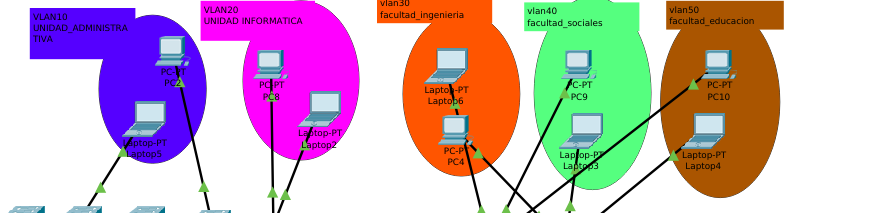
\includegraphics[scale=0.4]{img/vlans.png} 
\subsubsection{sede central administrativa}
Como en total tenemos 100 computadores, usaremos 5 switchs.
5 switchs = 120 puertos pero se usa 1 de cada switch para conectar al switch general que nos ayudará para poder expandir m\'as nuestra red en el futuro.
Entonces nos quedar\'ia 115 puertos(cada switch con 23 puertos utilizables)
\\
Usaremos 3 switchs completos para la VLAN10 unidad administrativa=69 + 11 puertos de un 4 switch=80 puertos configurados para VLAN10.
\\
Ya que en el switch 4 solo resta con 13(23-11) puertos lo mas ideal seria asignar 20 puertos del switch 5 a la VLAN20 unidad inform\'atica.

\\
\\
\textbf{CONFIGURAMOS LOS SWITCHS}

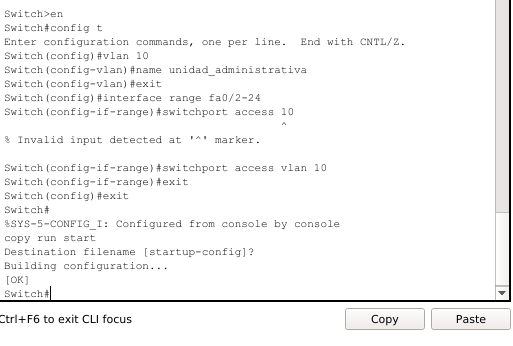
\includegraphics[scale=0.85]{img/switchvlan.png}
\\
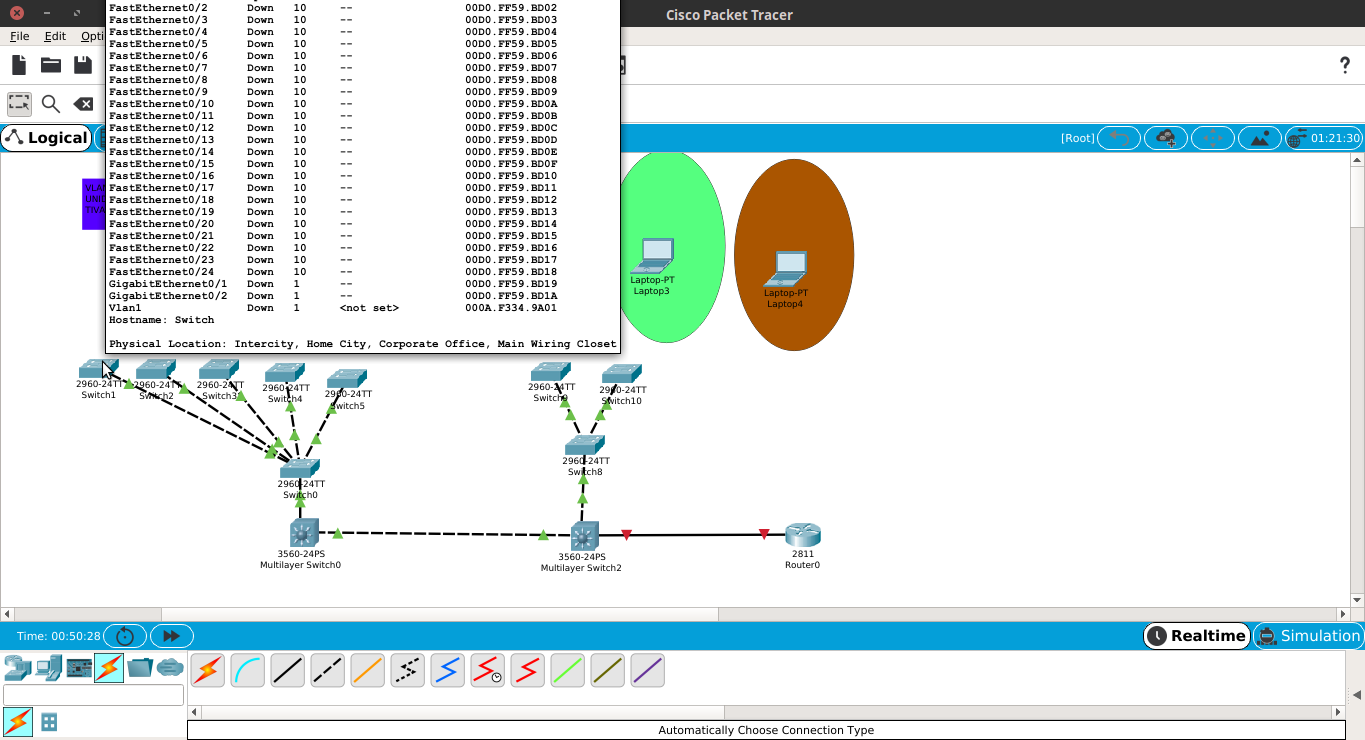
\includegraphics[scale=0.4]{img/vlan10.png} 
 \\\\
 y hacemos lo mismo con los dem\'as switchs.
 \\\\
 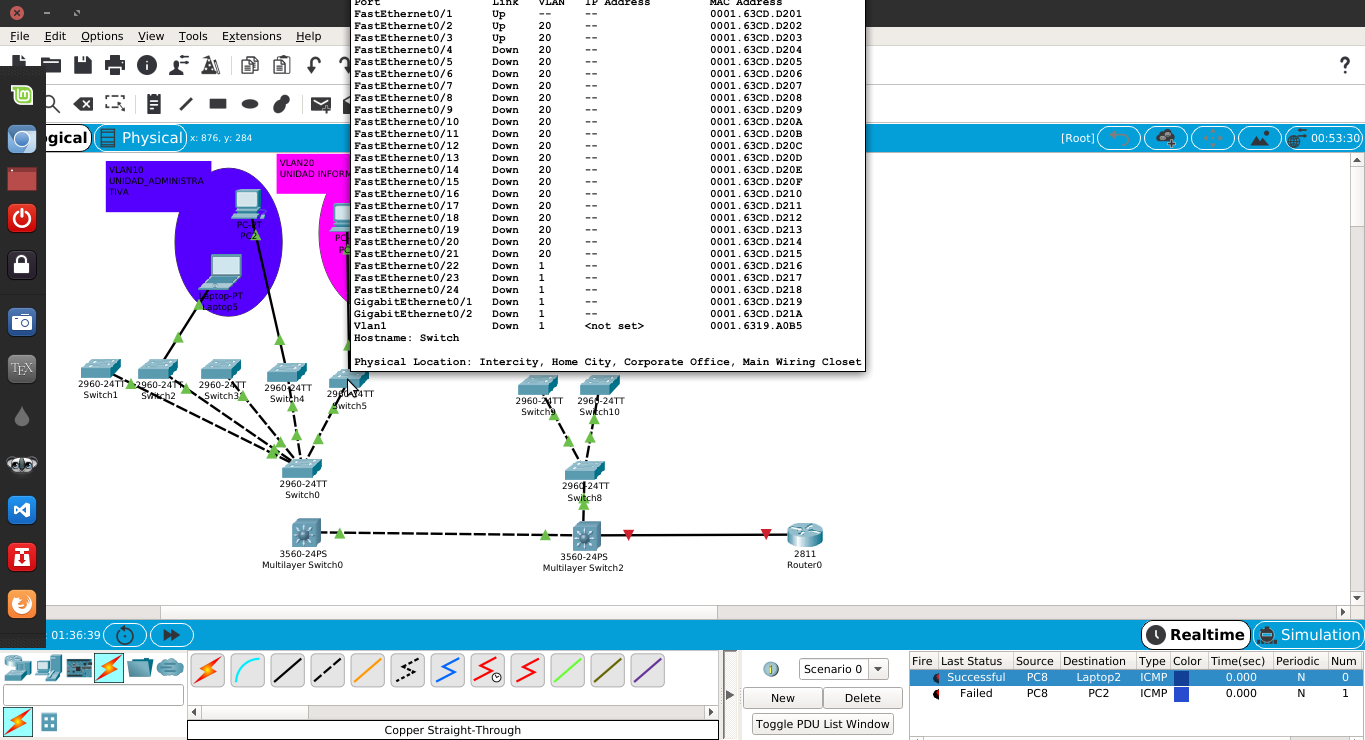
\includegraphics[scale=0.4]{img/vlan20.png} 
 
 \subsubsection{Campus Universitario}
 Para el campus universitario definiremos 3 vlans.
 para simplificar los procesos implementaremos solo 1 switch para cada edificio.
 como cada facultad se encuentra en cada edificio a cada uno le corresponder\'a un switch configurado como su vlan.
 
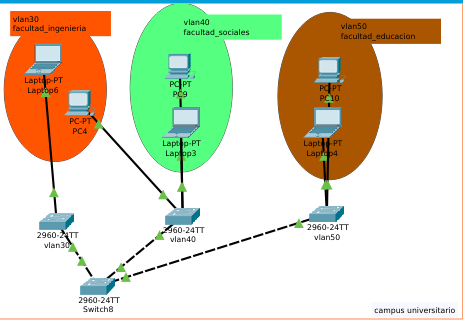
\includegraphics[scale=0.9]{img/campus.png} 
\subsection{Conexi\'on sucursal Lima}
para todas las sucursales para reducir el modelo a un modelo sencillo. asignamos dos switchs en el cual esta configurado las 3 vlans ya que solo existe un edificio en el que estudian los 3 estudiantes.
\subsubsection{sucursal cono norte}
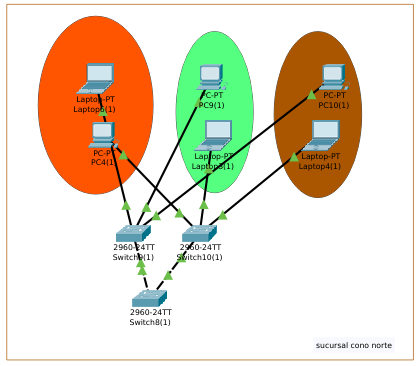
\includegraphics[scale=1]{img/cononorte.png} 
\subsubsection{sucursal cono centro}
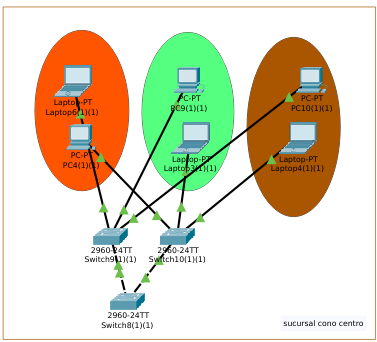
\includegraphics[scale=1]{img/conocentro.png} 
 \subsubsection{sucursal cono sur}
 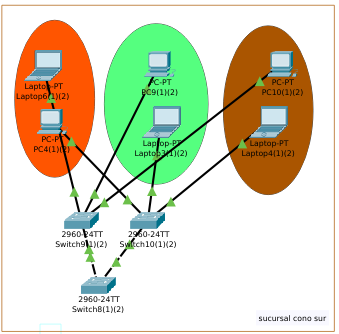
\includegraphics[scale=1]{img/conosur.png} 

\subsection{Conexi\'on sucursal Arequipa}
ser\'an de igual manera que de la sucursal de lima.
\\
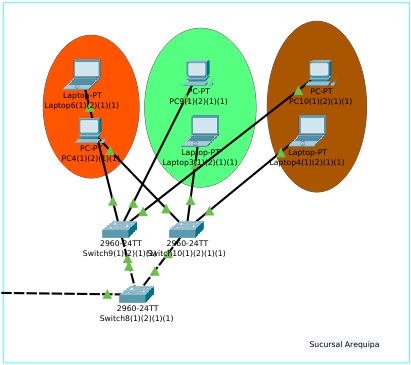
\includegraphics[scale=1]{img/arequipa.png} 
\subsection{Conexi\'on sucursal HUancayo}
ser\'an de igual manera que de la sucursal de lima.
\\
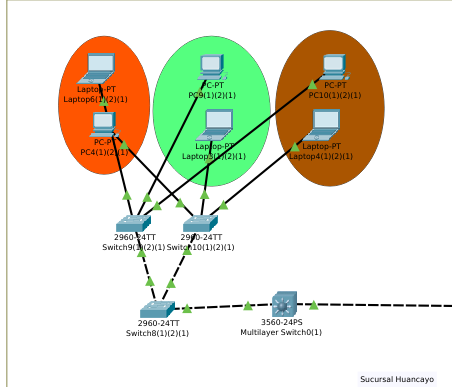
\includegraphics[scale=1]{img/huancayo.png} 

\section{\¿Le parece acertada la decisi\'on del Jefe de Inform\'atica?, Sustente en profundidad su respuesta para cada caso}
\subsection{SEGMENTACI\'ON DE REDES}
\begin{definicion}[]
{
\begin{enumerate}[label=\itembolasazules{}]
\item Qu\'e se adquiera una direcci\'on IP p\'ublica y que se utilice
segmentaci\'on basada en subredes IP para cada una de las sucursales.
\item Qu\'e cada una de las Facultades sean segmentadas utilizando VLAN.
\end{enumerate}
}
\end{definicion}}
Para este caso la utilizaci\'on de una ip publica mejora mucho la seguridad de una red ya que al salir hacia una wan o internet estamos propensos a sufrir suplantacion de identidad entre muchas otras cosas.
\\
la ip publica hace que esto sea mas dificil de realizar ya q siempre saldremos al exterior con una ip publica de conocimiento de todos.\\

NO solo las facultades deben de ser segmentadas en Vlans sino todas las unidades involucradas para poder tener asi un mejor control en la red.
\subsection{LOCALIZACI\'ON DE SERVIDORES}
\begin{definicion}[]
{
\begin{enumerate}[label=\itembolasazules{}]
\item Que la Oficina de Inform\'atica en Ayacucho tenga.

\begin{enumerate}[label=\itembolas{}]
\item 01 Servidor de DHCP, que asigne direcciones IP din\'amicas a las
sedes de Ayacucho, Arequipa y Huancayo.
\item 1 Servidor de DNS.
\item 1 Servidor Web que contenga las p\'aginas web de cada una de las
sedes (Ayacucho, Lima, Arequipa y Huancayo).
\end{enumerate}

\item Qu\'e la Sede Lima Cono Central tenga: 01 Servidor para servicio de DHCP, que asigne direcciones IP
din\'amicas a las tres sedes de Lima solamente.
\end{enumerate}
}

\end{definicion}}
Lo mas recomendable deber\'ia ser tener todos esos servidores en un ambiente m\'as adecuado, ya que no se menciona que la casona cuente con lo requerido para que se cumplan los est\'andares basicos que se requiere.
\\
Se deberia de separar con una granja de servidores y asi provea servicio a todos; los servidores deber\'ian de estar ubicados todos juntos en un lugar adecuado.

